\documentclass[tikz]{standalone}
\usepackage{xcolor}
\usetikzlibrary{matrix}
\usepackage{avant}
\definecolor{highlight}{RGB}{5,112,164}
\colorlet{nonmetal}{highlight!60}
\colorlet{metal}{highlight!20}
\colorlet{metaloid}{highlight!40}

\newcommand{\elementsquare}[8]{%
    \node[fill=#8, minimum width=2.4cm, minimum height=2.9cm, rounded corners] {};
    \node at (0, 0.4) {{\huge\textbf{#1}}};
    \node at (0, 0) {#2};
    \node[right] at (-1.1, 1.2) {\large\textbf{#3}};
    \node at (0, -0.4) {#4};
    \node at (0, -0.8) {#5};
    \node at (0, -1.2) {#6};
    \node[left] at (1.1, 1.2) {#7};
    \draw[white] (-1.3, -1.6) rectangle (1.3, 1.5);  % For spacing
}
% \elementsquare{symbol}{name}{atomic no}{mass no}{ground state electron config}{ionisation energy}{ground state}{colour}

\begin{document}
    \sffamily
    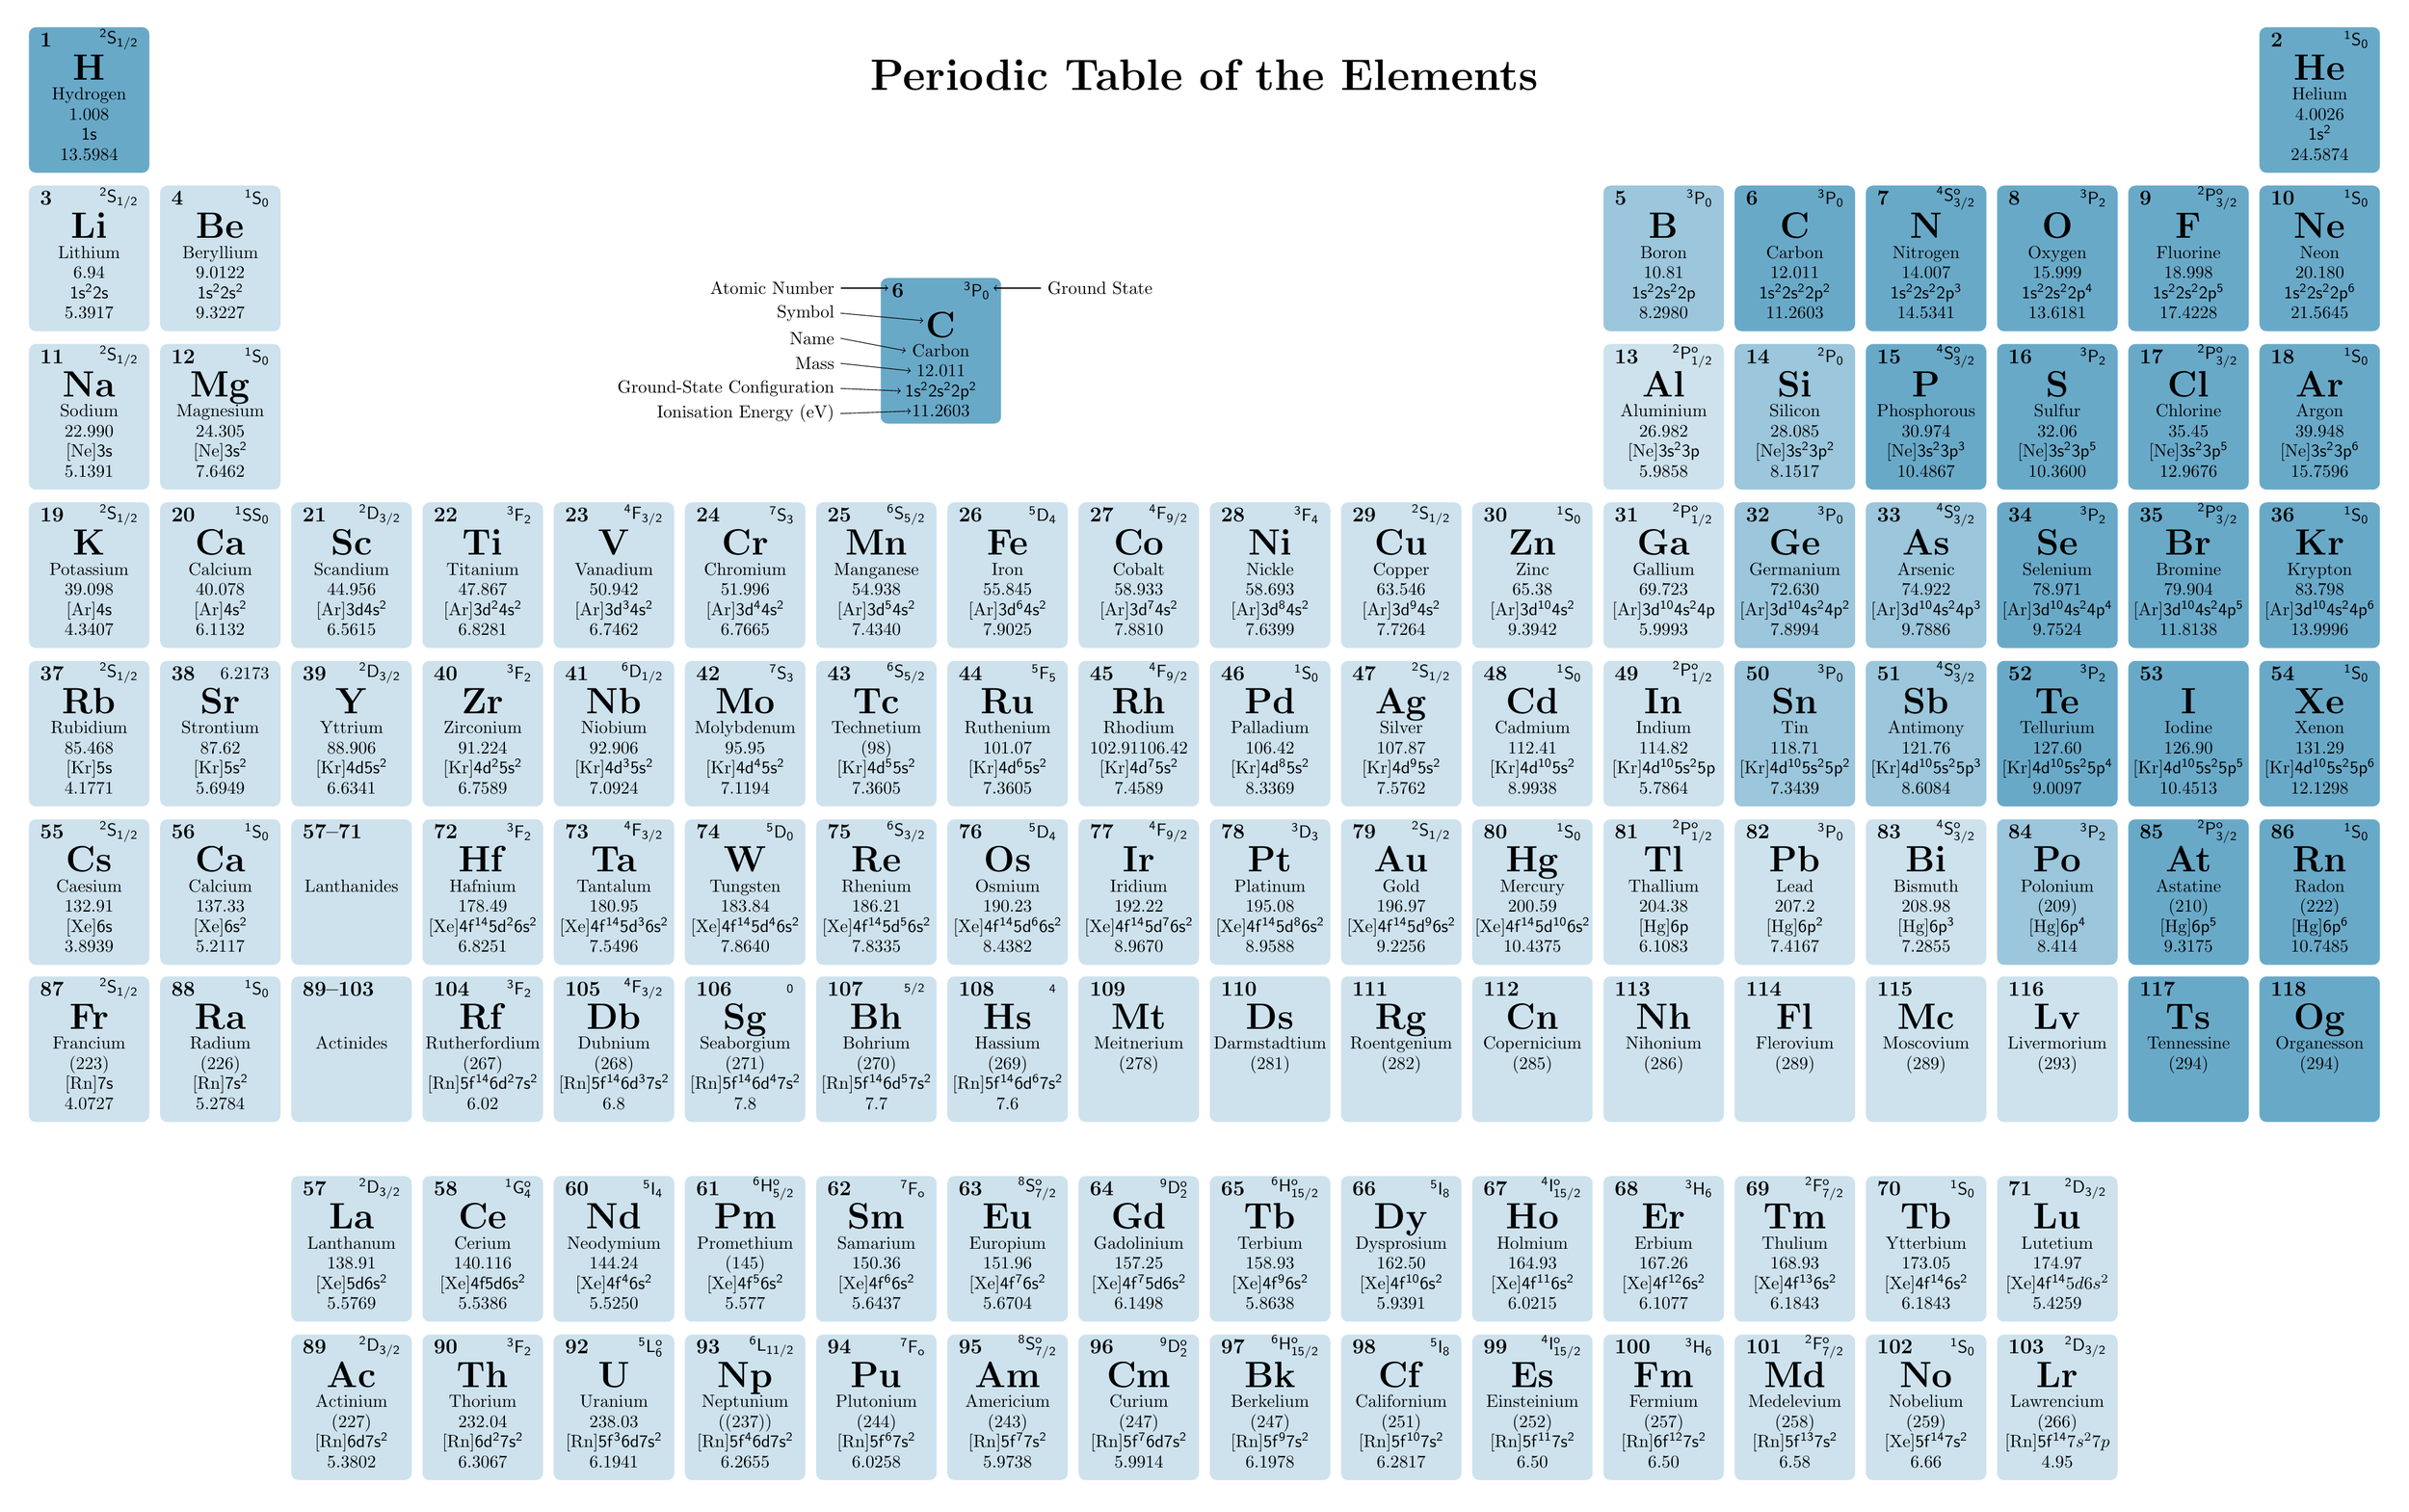
\begin{tikzpicture}
        \matrix [matrix of nodes] {
            % Hydrogen
            \elementsquare{H}{Hydrogen}{1}{1.008}{\(\mathsf{1s}\)}{13.5984}{\(\mathsf{^2S_{1/2}}\)}{nonmetal} &
            % Gaps
            &&&&&&&&&&&&&&&&
            % Helium
            \elementsquare{He}{Helium}{2}{4.0026}{\(\mathsf{1s^2}\)}{24.5874}{\(\mathsf{^1S_0}\)}{nonmetal} \\
            %
            % Lithium
            \elementsquare{Li}{Lithium}{3}{6.94}{\(\mathsf{1s^22s}\)}{5.3917}{\(\mathsf{^2S_{1/2}}\)}{metal} &
            % Beryllium
            \elementsquare{Be}{Beryllium}{4}{9.0122}{\(\mathsf{1s^22s^2}\)}{9.3227}{\(\mathsf{^1S_0}\)}{metal} &
            % Gaps
            &&&&&&&&&&
            % Boron
            \elementsquare{B}{Boron}{5}{10.81}{\(\mathsf{1s^22s^22p}\)}{8.2980}{\(\mathsf{^3P_0}\)}{metaloid} &
            % Carbon
            \elementsquare{C}{Carbon}{6}{12.011}{\(\mathsf{1s^22s^22p^2}\)}{11.2603}{\(\mathsf{^3P_0}\)}{nonmetal} &
            % Nitrogen
            \elementsquare{N}{Nitrogen}{7}{14.007}{\(\mathsf{1s^22s^22p^3}\)}{14.5341}{\(\mathsf{^4S_{3/2}^o}\)}{nonmetal} &
            % Oxygen
            \elementsquare{O}{Oxygen}{8}{15.999}{\(\mathsf{1s^22s^22p^4}\)}{13.6181}{\(\mathsf{^3P_2}\)}{nonmetal} &
            % Fluorine
            \elementsquare{F}{Fluorine}{9}{18.998}{\(\mathsf{1s^22s^22p^5}\)}{17.4228}{\(\mathsf{^2P_{3/2}^o}\)}{nonmetal} &
            % Neon
            \elementsquare{Ne}{Neon}{10}{20.180}{\(\mathsf{1s^22s^22p^6}\)}{21.5645}{\(\mathsf{^1S_0}\)}{nonmetal} \\
            %
            % Sodium
            \elementsquare{Na}{Sodium}{11}{22.990}{[Ne]\(\mathsf{3s}\)}{5.1391}{\(\mathsf{^2S_{1/2}}\)}{metal} &
            % Magnesium
            \elementsquare{Mg}{Magnesium}{12}{24.305}{[Ne]\(\mathsf{3s^2}\)}{7.6462}{\(\mathsf{^1S_0}\)}{metal} &
            % Gaps
            &&&&&&&&&&
            % Aluminium
            \elementsquare{Al}{Aluminium}{13}{26.982}{[Ne]\(\mathsf{3s^23p}\)}{5.9858}{\(\mathsf{^2P_{1/2}^o}\)}{metal} &
            % Silicon
            \elementsquare{Si}{Silicon}{14}{ 28.085}{[Ne]\(\mathsf{3s^23p^2}\)}{8.1517}{\(\mathsf{^2P_0}\)}{metaloid} &
            % Phosphorus
            \elementsquare{P}{Phosphorous}{15}{30.974}{[Ne]\(\mathsf{3s^23p^3}\)}{10.4867}{\(\mathsf{^4S_{3/2}^o}\)}{nonmetal} &
            % Sulfur
            \elementsquare{S}{Sulfur}{16}{ 32.06}{[Ne]\(\mathsf{3s^23p^5}\)}{10.3600}{\(\mathsf{^3P_2}\)}{nonmetal} &
            % Chlorine
            \elementsquare{Cl}{Chlorine}{17}{ 35.45}{[Ne]\(\mathsf{3s^23p^5}\)}{12.9676}{\(\mathsf{^2P_{3/2}^o}\)}{nonmetal} &
            % Argon
            \elementsquare{Ar}{Argon}{18}{39.948}{[Ne]\(\mathsf{3s^23p^6}\)}{15.7596}{\(\mathsf{^1S_0}\)}{nonmetal} \\
            %
            % Potassium
            \elementsquare{K}{Potassium}{19}{39.098}{[Ar]\(\mathsf{4s}\)}{4.3407}{\(\mathsf{^2S_{1/2}}\)}{metal} &
            % Calcium
            \elementsquare{Ca}{Calcium}{20}{40.078}{[Ar]\(\mathsf{4s^2}\)}{6.1132}{\(\mathsf{^1SS_0}\)}{metal} &
            % Scandium
            \elementsquare{Sc}{Scandium}{21}{44.956}{[Ar]\(\mathsf{3d4s^2}\)}{6.5615}{\(\mathsf{^2D_{3/2}}\)}{metal} &
            % Titanium
            \elementsquare{Ti}{Titanium}{22}{47.867}{[Ar]\(\mathsf{3d^24s^2}\)}{6.8281}{\(\mathsf{^3F_2}\)}{metal} &
            % Vanadium
            \elementsquare{V}{Vanadium}{23}{50.942}{[Ar]\(\mathsf{3d^34s^2}\)}{6.7462}{\(\mathsf{^4F_{3/2}}\)}{metal} &
            % Chromium
            \elementsquare{Cr}{Chromium}{24}{51.996}{[Ar]\(\mathsf{3d^44s^2}\)}{6.7665}{\(\mathsf{^7S_3}\)}{metal} &
            % Manganese
            \elementsquare{Mn}{Manganese}{25}{54.938}{[Ar]\(\mathsf{3d^54s^2}\)}{7.4340}{\(\mathsf{^6S_{5/2}}\)}{metal} &
            % Iron
            \elementsquare{Fe}{Iron}{26}{55.845}{[Ar]\(\mathsf{3d^64s^2}\)}{7.9025}{\(\mathsf{^5D_4}\)}{metal} &
            % Cobalt
            \elementsquare{Co}{Cobalt}{27}{58.933}{[Ar]\(\mathsf{3d^74s^2}\)}{7.8810}{\(\mathsf{^4F_{9/2}}\)}{metal} &
            % Nickel
            \elementsquare{Ni}{Nickle}{28}{58.693}{[Ar]\(\mathsf{3d^84s^2}\)}{7.6399}{\(\mathsf{^3F_4}\)}{metal} &
            % Copper
            \elementsquare{Cu}{Copper}{29}{63.546}{[Ar]\(\mathsf{3d^94s^2}\)}{7.7264}{\(\mathsf{^2S_{1/2}}\)}{metal} &
            % Zinc
            \elementsquare{Zn}{Zinc}{30}{65.38}{[Ar]\(\mathsf{3d^{10}4s^2}\)}{9.3942}{\(\mathsf{^1S_0}\)}{metal} &
            % Gallium
            \elementsquare{Ga}{Gallium}{31}{69.723}{[Ar]\(\mathsf{3d^{10}4s^24p}\)}{5.9993}{\(\mathsf{^2P_{1/2}^o}\)}{metal} &
            % Germanium
            \elementsquare{Ge}{Germanium}{32}{72.630}{[Ar]\(\mathsf{3d^{10}4s^24p^2}\)}{7.8994}{\(\mathsf{^3P_0}\)}{metaloid} &
            % Arsenic
            \elementsquare{As}{Arsenic}{33}{74.922}{[Ar]\(\mathsf{3d^{10}4s^24p^3}\)}{9.7886}{\(\mathsf{^4S_{3/2}^o}\)}{metaloid} &
            % Selenium
            \elementsquare{Se}{Selenium}{34}{78.971}{[Ar]\(\mathsf{3d^{10}4s^24p^4}\)}{9.7524}{\(\mathsf{^3P_2}\)}{nonmetal} &
            % Bromine
            \elementsquare{Br}{Bromine}{35}{79.904}{[Ar]\(\mathsf{3d^{10}4s^24p^5}\)}{11.8138}{\(\mathsf{^2P_{3/2}^o}\)}{nonmetal} &
            % Krypton
            \elementsquare{Kr}{Krypton}{36}{83.798}{[Ar]\(\mathsf{3d^{10}4s^24p^6}\)}{13.9996}{\(\mathsf{^1S_0}\)}{nonmetal} \\
            %
            % Rubidium
            \elementsquare{Rb}{Rubidium}{37}{85.468}{[Kr]\(\mathsf{5s}\)}{4.1771}{\(\mathsf{^2S_{1/2}}\)}{metal} &
            % Strontium
            \elementsquare{Sr}{Strontium}{38}{87.62}{[Kr]\(\mathsf{5s^2}\)}{5.6949}{6.2173}{metal} &
            % Yttrium
            \elementsquare{Y}{Yttrium}{39}{88.906}{[Kr]\(\mathsf{4d5s^2}\)}{6.6341}{\(\mathsf{^2D_{3/2}}\)}{metal} &
            % Zirconium
            \elementsquare{Zr}{Zirconium}{40}{91.224}{[Kr]\(\mathsf{4d^25s^2}\)}{6.7589}{\(\mathsf{^3F_2}\)}{metal} &
            % Niobium
            \elementsquare{Nb}{Niobium}{41}{92.906}{[Kr]\(\mathsf{4d^35s^2}\)}{7.0924}{\(\mathsf{^6D_{1/2}}\)}{metal} &
            % Molybdenum
            \elementsquare{Mo}{Molybdenum}{42}{95.95}{[Kr]\(\mathsf{4d^45s^2}\)}{7.1194}{\(\mathsf{^7S_3}\)}{metal} &
            % Technetium
            \elementsquare{Tc}{Technetium}{43}{(98)}{[Kr]\(\mathsf{4d^55s^2}\)}{7.3605}{\(\mathsf{^6S_{5/2}}\)}{metal} &
            % Ruthenium
            \elementsquare{Ru}{Ruthenium}{44}{101.07}{[Kr]\(\mathsf{4d^65s^2}\)}{7.3605}{\(\mathsf{^5F_5}\)}{metal} &
            % Rhodium
            \elementsquare{Rh}{Rhodium}{45}{102.91106.42}{[Kr]\(\mathsf{4d^75s^2}\)}{7.4589}{\(\mathsf{^4F_{9/2}}\)}{metal} &
            % Palladium
            \elementsquare{Pd}{Palladium}{46}{106.42}{[Kr]\(\mathsf{4d^85s^2}\)}{8.3369}{\(\mathsf{^1S_0}\)}{metal} &
            % Silver
            \elementsquare{Ag}{Silver}{47}{107.87}{[Kr]\(\mathsf{4d^95s^2}\)}{7.5762}{\(\mathsf{^2S_{1/2}}\)}{metal} &
            % Cadmium
            \elementsquare{Cd}{Cadmium}{48}{112.41}{[Kr]\(\mathsf{4d^{10}5s^2}\)}{8.9938}{\(\mathsf{^1S_0}\)}{metal} &
            % Indium
            \elementsquare{In}{Indium}{49}{114.82}{[Kr]\(\mathsf{4d^{10}5s^25p}\)}{5.7864}{\(\mathsf{^2P_{1/2}^o}\)}{metal} &
            % Tin
            \elementsquare{Sn}{Tin}{50}{118.71}{[Kr]\(\mathsf{4d^{10}5s^25p^2}\)}{7.3439}{\(\mathsf{^3P_0}\)}{metaloid} &
            % Antimony
            \elementsquare{Sb}{Antimony}{51}{121.76}{[Kr]\(\mathsf{4d^{10}5s^25p^3}\)}{8.6084}{\(\mathsf{^4S_{3/2}^o}\)}{metaloid} &
            % Tellurium
            \elementsquare{Te}{Tellurium}{52}{127.60}{[Kr]\(\mathsf{4d^{10}5s^25p^4}\)}{9.0097}{\(\mathsf{^3P_2}\)}{nonmetal} &
            % Iodine
            \elementsquare{I}{Iodine}{53}{126.90}{[Kr]\(\mathsf{4d^{10}5s^25p^5}\)}{10.4513}{}{nonmetal} &
            % Xenon
            \elementsquare{Xe}{Xenon}{54}{ 131.29}{[Kr]\(\mathsf{4d^{10}5s^25p^6}\)}{12.1298}{\(\mathsf{^1S_0}\)}{nonmetal} \\
            %
            % Caesium
            \elementsquare{Cs}{Caesium}{55}{132.91}{[Xe]\(\mathsf{6s}\)}{3.8939}{\(\mathsf{^2S_{1/2}}\)}{metal} &
            % Barium
            \elementsquare{Ca}{Calcium}{56}{137.33}{[Xe]\(\mathsf{6s^2}\)}{5.2117}{\(\mathsf{^1S_0}\)}{metal} &
            % Skip
            \elementsquare{}{Lanthanides}{57--71}{}{}{}{}{metal} &
            % Hafnium
            \elementsquare{Hf}{Hafnium}{72}{178.49}{[Xe]\(\mathsf{4f^{14}5d^26s^2}\)}{6.8251}{\(\mathsf{^3F_2}\)}{metal} &
            % Tantalum
            \elementsquare{Ta}{Tantalum}{73}{180.95}{[Xe]\(\mathsf{4f^{14}5d^36s^2}\)}{7.5496}{\(\mathsf{^4F_{3/2}}\)}{metal} &
            % Tungsten
            \elementsquare{W}{Tungsten}{74}{183.84}{[Xe]\(\mathsf{4f^{14}5d^46s^2}\)}{7.8640}{\(\mathsf{^5D_0}\)}{metal} &
            % Rhenium
            \elementsquare{Re}{Rhenium}{75}{186.21}{[Xe]\(\mathsf{4f^{14}5d^56s^2}\)}{7.8335}{\(\mathsf{^6S_{3/2}}\)}{metal} &
            % Osmium
            \elementsquare{Os}{Osmium}{76}{190.23}{[Xe]\(\mathsf{4f^{14}5d^66s^2}\)}{8.4382}{\(\mathsf{^5D_4}\)}{metal} &
            % Iridium
            \elementsquare{Ir}{Iridium}{77}{192.22}{[Xe]\(\mathsf{4f^{14}5d^76s^2}\)}{8.9670}{\(\mathsf{^4F_{9/2}}\)}{metal} &
            % Platinum
            \elementsquare{Pt}{Platinum}{78}{195.08}{[Xe]\(\mathsf{4f^{14}5d^86s^2}\)}{8.9588}{\(\mathsf{^3D_3}\)}{metal} &
            % Gold
            \elementsquare{Au}{Gold}{79}{196.97}{[Xe]\(\mathsf{4f^{14}5d^96s^2}\)}{9.2256}{\(\mathsf{^2S_{1/2}}\)}{metal} &
            % Mercury
            \elementsquare{Hg}{Mercury}{80}{200.59}{[Xe]\(\mathsf{4f^{14}5d^{10}6s^2}\)}{10.4375}{\(\mathsf{^1S_0}\)}{metal} &
            % Thallium
            \elementsquare{Tl}{Thallium}{81}{  204.38}{[Hg]\(\mathsf{6p}\)}{6.1083}{\(\mathsf{^2P_{1/2}^o}\)}{metal} &
            % Lead
            \elementsquare{Pb}{Lead}{82}{207.2}{[Hg]\(\mathsf{6p^2}\)}{7.4167}{\(\mathsf{^3P_0}\)}{metal} &
            % Bismuth
            \elementsquare{Bi}{Bismuth}{83}{208.98}{[Hg]\(\mathsf{6p^3}\)}{7.2855}{\(\mathsf{^4S_{3/2}^o}\)}{metal} &
            % Polonium
            \elementsquare{Po}{Polonium}{84}{(209)}{[Hg]\(\mathsf{6p^4}\)}{8.414}{\(\mathsf{^3P_2}\)}{metaloid} &
            % Astatine
            \elementsquare{At}{Astatine}{85}{(210)}{[Hg]\(\mathsf{6p^5}\)}{9.3175}{\(\mathsf{^2P_{3/2}^o}\)}{nonmetal} &
            % Radon
            \elementsquare{Rn}{Radon}{86}{(222)}{[Hg]\(\mathsf{6p^6}\)}{10.7485}{\(\mathsf{^1S_0}\)}{nonmetal} \\
            %
            % Francium
            \elementsquare{Fr}{Francium}{87}{(223)}{[Rn]\(\mathsf{7s}\)}{4.0727}{\(\mathsf{^2S_{1/2}}\)}{metal} &
            % Radium
            \elementsquare{Ra}{Radium}{88}{(226)}{[Rn]\(\mathsf{7s^2}\)}{5.2784}{\(\mathsf{^1S_0}\)}{metal} &
            % Skip
            \elementsquare{}{Actinides}{89--103}{}{}{}{}{metal} &
            % Rutherfordium
            \elementsquare{Rf}{Rutherfordium}{104}{(267)}{[Rn]\(\mathsf{5f^{14}6d^27s^2}\)}{6.02}{\(\mathsf{^3F_2}\)}{metal} &
            % Dubnium
            \elementsquare{Db}{Dubnium}{105}{(268)}{[Rn]\(\mathsf{5f^{14}6d^37s^2}\)}{6.8}{\(\mathsf{^4F_{3/2}}\)}{metal} &
            % Seaborgium
            \elementsquare{Sg}{Seaborgium}{106}{(271)}{[Rn]\(\mathsf{5f^{14}6d^47s^2}\)}{7.8}{\(\mathsf{_0}\)}{metal} &
            % Bohrium
            \elementsquare{Bh}{Bohrium}{107}{(270)}{[Rn]\(\mathsf{5f^{14}6d^57s^2}\)}{7.7}{\(\mathsf{_{5/2}}\)}{metal} &
            % Hassium
            \elementsquare{Hs}{Hassium}{108}{(269)}{[Rn]\(\mathsf{5f^{14}6d^67s^2}\)}{7.6}{\(\mathsf{_4}\)}{metal} &
            % Meitnerium
            \elementsquare{Mt}{Meitnerium}{109}{(278)}{}{}{}{metal} &
            % Darmstadtium
            \elementsquare{Ds}{Darmstadtium}{110}{(281)}{}{}{}{metal} &
            % Roentgenium
            \elementsquare{Rg}{Roentgenium}{111}{(282)}{}{}{}{metal} &
            % Copernicium
            \elementsquare{Cn}{Copernicium}{112}{(285)}{}{}{}{metal} &
            % Nihonium
            \elementsquare{Nh}{Nihonium}{113}{(286)}{}{}{}{metal} &
            % Flerovium
            \elementsquare{Fl}{Flerovium}{114}{(289)}{}{}{}{metal} &
            % Moscovium
            \elementsquare{Mc}{Moscovium}{115}{(289)}{}{}{}{metal} &
            % Livermorium
            \elementsquare{Lv}{Livermorium}{116}{(293)}{}{}{}{metal} &
            % Tennessine
            \elementsquare{Ts}{Tennessine}{117}{(294)}{}{}{}{nonmetal} &
            % Organesson
            \elementsquare{Og}{Organesson}{118}{(294)}{}{}{}{nonmetal} \\
        };
        \begin{scope}[yshift=-15cm]
            \matrix [matrix of nodes] {
                % Lanthanum
                \elementsquare{La}{Lanthanum}{57}{138.91}{[Xe]\(\mathsf{5d6s^2}\)}{5.5769}{\(\mathsf{^2D_{3/2}}\)}{metal} & 
                % Cerium
                \elementsquare{Ce}{Cerium}{58}{140.116}{[Xe]\(\mathsf{4f5d6s^2}\)}{5.5386}{\(\mathsf{^1G_4^o}\)}{metal} &
                % Praseodymium
                \elementsquare{Pr}{Praseodymium}{59}{140.91}{[Xe]\(\mathsf{4f^36s^2}\)}{5.4702}{\(\mathsf{^4I_{3/2}^o}\)}{metal}
                % Neodymium
                \elementsquare{Nd}{Neodymium}{60}{144.24}{[Xe]\(\mathsf{4f^46s^2}\)}{5.5250}{\(\mathsf{^5I_4}\)}{metal} & 
                % Promethium
                \elementsquare{Pm}{Promethium}{61}{(145)}{[Xe]\(\mathsf{4f^56s^2}\)}{5.577}{\(\mathsf{^6H_{5/2}^o}\)}{metal} & 
                % Samarium
                \elementsquare{Sm}{Samarium}{62}{150.36}{[Xe]\(\mathsf{4f^66s^2}\)}{5.6437}{\(\mathsf{^7F_o}\)}{metal} &
                % Europium
                \elementsquare{Eu}{Europium}{63}{151.96}{[Xe]\(\mathsf{4f^76s^2}\)}{5.6704}{\(\mathsf{^8S_{7/2}^o}\)}{metal} & 
                % Gadolinium
                \elementsquare{Gd}{Gadolinium}{64}{157.25}{[Xe]\(\mathsf{4f^75d6s^2}\)}{6.1498}{\(\mathsf{^9D_2^o}\)}{metal} & 
                % Terbium
                \elementsquare{Tb}{Terbium}{65}{158.93}{[Xe]\(\mathsf{4f^96s^2}\)}{5.8638}{\(\mathsf{^6H_{15/2}^o}\)}{metal} &
                % Dysprosium
                \elementsquare{Dy}{Dysprosium}{66}{162.50}{[Xe]\(\mathsf{4f^{10}6s^2}\)}{5.9391}{\(\mathsf{^5I_8}\)}{metal} &
                % Holmium
                \elementsquare{Ho}{Holmium}{67}{164.93}{[Xe]\(\mathsf{4f^{11}6s^2}\)}{6.0215}{\(\mathsf{^4I_{15/2}^o}\)}{metal} &
                % Erbium
                \elementsquare{Er}{Erbium}{68}{167.26}{[Xe]\(\mathsf{4f^{12}6s^2}\)}{6.1077}{\(\mathsf{^3H_6}\)}{metal} & 
                % Thulium
                \elementsquare{Tm}{Thulium}{69}{168.93}{[Xe]\(\mathsf{4f^{13}6s^2}\)}{6.1843}{\(\mathsf{^2F_{7/2}^o}\)}{metal} &
                % Ytterbium
                \elementsquare{Tb}{Ytterbium}{70}{173.05}{[Xe]\(\mathsf{4f^{14}6s^2}\)}{6.1843}{\(\mathsf{^1S_0}\)}{metal} & 
                % Lutetium
                \elementsquare{Lu}{Lutetium}{71}{174.97}{[Xe]\(\mathsf{4f^{14}}5d6s^2\)}{5.4259}{\(\mathsf{^2D_{3/2}}\)}{metal} \\
                %
                % Actinium
                \elementsquare{Ac}{Actinium}{89}{(227)}{[Rn]\(\mathsf{6d7s^2}\)}{5.3802}{\(\mathsf{^2D_{3/2}}\)}{metal} & 
                % Thorium
                \elementsquare{Th}{Thorium}{90}{232.04}{[Rn]\(\mathsf{6d^27s^2}\)}{6.3067}{\(\mathsf{^3F_2}\)}{metal} &
                % Protactinium
                \elementsquare{Ra}{Protactinium}{91}{231.04}{[Rn]\(\mathsf{5f^26d7s^2}\)}{5.89}{\(\mathsf{^4I_{11/2}^o}\)}{metal}
                % Uranium
                \elementsquare{U}{Uranium}{92}{238.03}{[Rn]\(\mathsf{5f^36d7s^2}\)}{6.1941}{\(\mathsf{^5L_6^o}\)}{metal} & 
                % Neptunium
                \elementsquare{Np}{Neptunium}{93}{((237))}{[Rn]\(\mathsf{5f^46d7s^2}\)}{6.2655}{\(\mathsf{^6L_{11/2}}\)}{metal} & 
                % Plutonium
                \elementsquare{Pu}{Plutonium}{94}{(244)}{[Rn]\(\mathsf{5f^67s^2}\)}{6.0258}{\(\mathsf{^7F_o}\)}{metal} &
                % Americium
                \elementsquare{Am}{Americium}{95}{(243)}{[Rn]\(\mathsf{5f^77s^2}\)}{5.9738}{\(\mathsf{^8S_{7/2}^o}\)}{metal} & 
                % Curium
                \elementsquare{Cm}{Curium}{96}{(247)}{[Rn]\(\mathsf{5f^76d7s^2}\)}{5.9914}{\(\mathsf{^9D_2^o}\)}{metal} & 
                % Berkelium
                \elementsquare{Bk}{Berkelium}{97}{(247)}{[Rn]\(\mathsf{5f^97s^2}\)}{6.1978}{\(\mathsf{^6H_{15/2}^o}\)}{metal} &
                % Californium
                \elementsquare{Cf}{Californium}{98}{(251)}{[Rn]\(\mathsf{5f^{10}7s^2}\)}{6.2817}{\(\mathsf{^5I_8}\)}{metal} &
                % Einsteinium
                \elementsquare{Es}{Einsteinium}{99}{(252)}{[Rn]\(\mathsf{5f^{11}7s^2}\)}{6.50}{\(\mathsf{^4I_{15/2}^o}\)}{metal} &
                % Fermium
                \elementsquare{Fm}{Fermium}{100}{(257)}{[Rn]\(\mathsf{6f^{12}7s^2}\)}{6.50}{\(\mathsf{^3H_6}\)}{metal} & 
                % Mendelevium
                \elementsquare{Md}{Medelevium}{101}{(258)}{[Rn]\(\mathsf{5f^{13}7s^2}\)}{6.58}{\(\mathsf{^2F_{7/2}^o}\)}{metal} &
                % Nobelium
                \elementsquare{No}{Nobelium}{102}{(259)}{[Xe]\(\mathsf{5f^{14}7s^2}\)}{6.66}{\(\mathsf{^1S_0}\)}{metal} & 
                % Lawrencium
                \elementsquare{Lr}{Lawrencium}{103}{(266)}{[Rn]\(\mathsf{5f^{14}}7s^27p\)}{4.95}{\(\mathsf{^2D_{3/2}}\)}{metal} \\
            };
            \end{scope}
            
            \begin{scope}[yshift=4.5cm, xshift=-5.25cm]
            \elementsquare{\raisebox{0.75ex}{C}}{Carbon}{6}{12.011}{\(\mathsf{1s^22s^22p^2}\)}{11.2603}{\(\mathsf{^3P_0}\)}{nonmetal}
            \node[left] at (-2, 1.25) {Atomic Number};
            \node[left] at (-2, 0.75) {Symbol};
            \node[left] at (-2, 0.25) {Name};
            \node[left] at (-2, -0.25) {Mass};
            \node[left] at (-2, -0.75) {Ground-State Configuration};
            \node[left] at (-2, -1.25) {Ionisation Energy (eV)};
            % TODO: Change eV to proper siunitx units syntax
            \node[right] at (2, 1.25) {Ground State};
            
            \draw[->] (-2, 1.25) -- (-1.05, 1.25);
            \draw[->] (-2, 0.75) -- (-0.35, 0.6);
            \draw[->] (-2, 0.25) -- (-0.7, 0);
            \draw[->] (-2, -0.25) -- (-0.6, -0.4);
            \draw[->] (-2, -0.75) -- (-0.8, -0.8);
            \draw[->] (-2, -1.25) -- (-0.6, -1.2);
            \draw[->] (2, 1.25) -- (1.05, 1.25);
        \end{scope}
        
        \node at (0, 10) {{\Huge\textbf{Periodic Table of the Elements}}};
    \end{tikzpicture}
\end{document}